\chapter{The LHC and the CMS experiment} \label{chap:LHCCMS}
\section{The LHC} \label{sec:LHCCMS_LHC}
The Large Hadron Collider (LHC)~\cite{ref:1748-0221/3/08/S08001} at CERN is, as the name suggests, the world's largest
and most powerful particle accelerator. It is used to collide protons as well as heavy ions, which are both examples of hadrons, hence the ``HC'' in LHC.
Experiments attached to the collider examine the collision debris, from which features of the
parent hard-scattering process may be inferred, allowing models such as those described in Chap.~\ref{chap:introduction} to be tested.

The collider consists of a closed loop of beam pipes, along with its RF cavities (sec.~\ref{sec:LHCCMS_LHC_proton_acceleration}), magnets,
and cryogenic and vacuum systems. It sits in a circular tunnel 26.7\unit{km} in circumference, lying between 45 and 170\unit{m} underground, straddling
the French--Swiss border near Geneva, Switzerland. The beam pipes are subdivided into eight straight and eight arc sections, forming a rounded octagon.
To orient navigation, there are eight designated points spaced evenly around the tunnel perimeter, one in the middle of each 8528\unit{m}-long straight section.
The four main LHC experiments surround the LHC beam pipe at four of these points: ATLAS~\cite{ref:10.1088/1748-0221/3/08/S08003}
at point 1, ALICE~\cite{ref:1748-0221/3/08/S08002} at point 2, CMS~\cite{ref:1748-0221/3/08/S08004} at point 5, and LHCb~\cite{ref:1748-0221/3/08/S08005} at point 8.
Their arrangement is shown in Fig.~\ref{fig:LHC_schematic}.

\begin{figure}[hbtp]
  \begin{center}
    \includegraphics[width=0.70\textwidth]{Figures/Schematic-layout-of-the-LHC-at-CERN.png}
    \caption{
    Schematic layout of the LHC, from~\cite{ref:PhysRevAccelBeams.20.091002}.
    }
    \label{fig:LHC_schematic}
  \end{center}
\end{figure}

The eight arc sections are each filled with a series of dipole bending magnets, 1232 in all. When a current is run through them, these produce a uniform magnetic
field inside their segments of the beam pipes, pointing perpendicular to the beam direction.
A magnetic field causes a charged particle's trajectory to bend, and the dipoles are arranged so as to keep the proton beam trajectories aligned with the beam pipes
throughout the arcs.
Since a fixed magnetic field causes protons moving in opposite directions to bend in opposite directions, the two counter-rotating beams must be deflected by oppositely-aligned fields.
A special two-in-one magnet design was developed for the LHC that produces two side-by-side dipole fields, coupled to the same current, oriented in opposite directions. The use of
superconducting NbTi cables allows more than 12\unit{kA} to flow when the wire is cooled to 1.9\unit{K}, producing a dipole field of up to 9\unit{T}. Sophisticated cryogenic and power
transmission systems are required to operate the magnets at this level, and the two-in-one design prevents each pipe from needing its own separate system along more than 18\unit{km} of
total dipole magnet length, substantially reducing the space and cost requirements of the LHC.

The arc dipoles each have a radius of curvature $R = 2.804\unit{km}$. This radius constrains the energy of a relativistic particle
bent in a circular trajectory by a magnetic field of magnitude $B$, via the relation~\cite{ref:WilleAccelerators}
\begin{equation}
E = qcBR
\end{equation}
where $q$ is the particle's electric charge and $c$ is the speed of light. For a fixed
particle type and magnet strength, $E$ is directly proportional to $R$. Accordingly, higher-energy
colliders tend to be built with larger circumferences than lower-energy colliders.
The energy of a fully-accelerated LHC proton in 2016 was 6.5\unit{TeV}, corresponding to a dipole field of 7.7\unit{T}.

Smaller accelerators including the Proton Synchrotron (PS) and Super Proton Synchrotron (SPS) used to be flagship accelerators
in their own right, but now chiefly serve as intermediate stages in an accelerator complex that feeds the LHC.
The LHC itself occupies the tunnel originally dug to house the Large Electron-Positron (LEP) collider~\cite{ref:SchopperLEP}, which collided
electrons and their antipartners (positrons) and ran from 1989 until 2000, setting some of the original results
listed in Chap.~\ref{chap:introduction}. The Fermilab Tevatron~\cite{ref:TevatronPhysics}, which ran from 1983 to 2011, occupied a smaller tunnel
but achieved higher energies than LEP by accelerating heavier particles: protons and their antipartners\footnote{These and other recent collider
experiments are reviewed in~\cite{ref:PDG}, chapter 30.}. The LHC, inaugurated in 2008,
accelerates protons in the world's largest accelerator tunnel, with state-of-the-art bending
magnets, allowing it to achieve unprecedented particle collision energies.

\subsection{Proton acceleration and collision} \label{sec:LHCCMS_LHC_proton_acceleration}
In practice, a low-energy proton beam is too wide to inject directly into the LHC beam pipes, but the beam can be narrowed by accelerating it~\cite{ref:PartPhysLHCEra}.
The beam is therefore passed through a chain of several different accelerators before ultimately arriving at the LHC.
Protons are initially collected by ionizing hydrogen gas, and as of 2016 they are fed to the LINAC2, a linear accelerator which accelerates
them to 50\unit{MeV} before sending them to the PS booster, which brings them up to 1.4\unit{GeV}. The protons are then sent to the PS, taking them to 25\unit{GeV},
and after that to the SPS, which pushes them to 450\unit{GeV} before finally injecting them into the LHC for final acceleration up to 6.5\unit{TeV}.

Protons are accelerated by passing through radio-frequency (RF) cavities, which generate oscillating electromagnetic
fields. Forward acceleration only results if the proton passes through the RF cavity at an opportune point in its oscillation cycle.
Thus, rather than circulating in a continuous beam, protons are segregated into discrete \textit{bunches}. In the LHC, the RF
frequency is tuned to 400.790\unit{MHz}, and bunches are spaced so as to keep 10 RF oscillations between each bunch. This corresponds
to a minimum bunch separation of 24.95\unit{ns} in time, with enough length in the tunnel to fit exactly 3564 bunches, each orbiting
with a frequency $f_\mathrm{rev} = 11.245\unit{kHz}$. A maximum of
2808 bunches can be injected in practice, to allow a sufficiently long empty interval for the beam injection and beam dump
redirector magnets to activate, and also respecting constraints imposed by assembling the bunch trains via the accelerator chain.
Beam optimization strategies and other operational constraints, including a persistent vacuum leak in the SPS beam dump
during 2016, can reduce this further. In 2016, the typical number of bunches per beam $n_b$ was 2076.

Two separate bunch trains counter-rotate around the LHC in separate beam pipes, with their paths crossing at four collision points
corresponding to each of the main experiments. The center-of-mass collision energy of the beams, $\sqrt{s}$, is twice that of the
individual beam energies. For a single-beam energy of 6.5\unit{TeV}, this corresponds to $\sqrt{s} = 13\unit{TeV}$.
Each bunch contains many billions of protons: in 2016, the typical number of protons per bunch at the start of each fill, $N_b$, was $1.25 \times 10^{11}$.
As a consequence, many pairs of protons can undergo hard collisions within the same
bunch crossing, depending on the instantaneous luminosity $\mathcal{L}$ and the total inelastic \Pp\Pp\ scattering cross section $\sigma_\mathrm{inel}$.
In 2016, there were on average 23 of these \textit{pileup} collisions per bunch crossing.

Various parameters describing the geometric profile of the bunches
are listed in Table~\ref{tab:beam_geo}. These determine $\mathcal{L}$ at the collision points, via
\begin{equation}
\mathcal{L} = \frac{N_{b}^{2}n_{b}f_\mathrm{rev}\gamma_{r}}{4\pi\epsilon_{n}\beta^\mathrm{*}}\left(1 + \frac{\theta_{c}^{2}\sigma_{z}^{2}\gamma_{r}}{4\epsilon_{n}\beta^\mathrm{*}}\right)^{-1/2}
\label{eq:instantaneous_lumi}
\end{equation}
in which the relativistic factor $\gamma_{r} = E_\mathrm{beam}/m_{p}$ has a value of 6930 for $E_\mathrm{beam} = 6.5\unit{TeV}$.
The value of $\mathcal{L}$ corresponding to the typical 2016 parameter values listed above is $1.3 \times 10^{34}$ $\mathrm{cm}^{-2}\mathrm{s}^{-1}$.

\begin{table}
\centering
\begin{tabular}{ cc }
\hline
Normalized transverse emittance $\epsilon_{n}$ & 3.4\unit{\micro m} \\
$\beta^{*}$ & 40\unit{cm} \\
Crossing angle $\theta_{c}$ & 185\unit{\micro rad} \\
RMS longitudinal bunch length $\sigma_{z}$ & 7.87\unit{cm} \\
\hline
\end{tabular}
\caption{Beam geometry parameters for 2016}
\label{tab:beam_geo}
\end{table}

\subsection{Collimation, magnets, and beam halo} \label{sec:LHCCMS_LHC_magnets_beam_halo}
The beams can lose protons during transit through a variety of mechanisms, such as intra-beam scattering
and scattering off of residual gas inside the tunnel~\cite{ref:1748-0221/3/08/S08001}. Among other consequences, this leads
to the accumulation of a ``halo'' of protons with large radial separation from the central beam axis, accompanying the main beam.
If left unchecked, beam halo could damage unprotected equipment and leave spurious signals in detectors.
Furthermore, if a bending magnet were to suddenly fail, the beam would sweep across the area downstream of the magnet, dumping a potentially
devastating load of radiation on whatever it hit.

Collimators stationed around the beam line capture and remove this halo,
and additionally protect the LHC and its detectors from sudden beam control failure.
Every proton--collimator interaction produces a residual shower of secondary particles that emerge from the other side of the collimator
and continue forward, so a series of several collimators is required.
Primary LHC collimators (TCP) clean the beam at Points 3 and 7, and secondary collimators (TCS) catch most of the output from those.
Tertiary collimators (TCT) made of a heavy tungsten alloy sit on either side of the CMS experimental cavern,
to scrub as much remaining halo as possible before it reaches the detector~\cite{ref:PhysRevAccelBeams.20.091002}.

As noted above, a series of 1232 main dipole magnets spaced around the LHC keep the beams moving
in their quasi-circular trajectories around the tunnel. A multitude of other magnets serve more specialized roles. Quadrupole
magnets have the effect of squeezing the beam along one axis and stretching it along another, and are used to focus
the beam along a specific direction. Near the interaction point (IP) of each experiment, an inner triplet of quadrupole magnets
are the last to interact with the beams before they collide. Figure~\ref{fig:magnet_positions} shows the arrangement
of magnets near the ATLAS and CMS IPs.

\begin{figure}[hbtp]
  \begin{center}
    \includegraphics[width=0.80\textwidth]{Figures/magnet_positions.png}
    \caption{
    Dipole (D1-2) and quadrupole (Q1-7) magnet arrangement near the left side of the IP, from~\cite{ref:PAC.2003.1289077}.
    This arrangement is mirrored on the right side of the IP.
    The figure specifically designates IP1, the ATLAS IP; the magnet layout is identical around IP5, the CMS IP.
    The inner triplet of quadrupole magnets (with two varieties, designated MQXA and MQXB)
    are the last to interact with the beam before collision.
    The distance from the left edge of Q3 (MQXA) to the IP is about 53\unit{m},
    and the distance from the right edge of Q1 to the IP is about 23\unit{m}.
    The TCT sits between D2 and TAN, about 150\unit{m} from the IP.
    }
    \label{fig:magnet_positions}
  \end{center}
\end{figure}

The envelope of each beam reaches a maximum in the inner triplet
before finally being focused toward a minimum at the interaction point. Beam halo is correspondingly widely dispersed,
and the TCTs are specifically placed about 150\unit{m} out from the IP so as to protect the inner triplet from this halo~\cite{ref:PhysRevSTAB.18.061001}.
Secondary particles produced from beam
halo collisions with the TCTs include large numbers of high-energy muons, along with an assortment of other secondaries.
These, along with the secondaries from proton collisions with residual gas in the beam pipe, comprise
what is called the machine-induced background (MIB) impinging on CMS~\cite{ref:1748-0221/10/11/P11011}.

In contrast to protons in the beam, secondary muons are neither narrowly nor evenly focused by the final stretch of magnets before reaching the IP.
They enter the CMS cavern traveling parallel to the beam pipe with a wide radial profile, often having a high enough
radius to hit the exterior muon chambers and calorimeters~\cite{ref:1748-0221/10/11/P11011}.
Furthermore, the transverse distribution of MIB (Fig.~\ref{fig:beamhalo_sim}) is highly anisotropic, concentrating near the
horizontal plane. Every other process examined in this thesis produces a distribution of events with constant density as a function
of angle around the beamline, and so the unique angular distribution of MIB is used to estimate its likely preponderance in a set of collision
events.

\begin{figure}[hbtp]
  \begin{center}
    \includegraphics[width=0.50\textwidth]{Figures/beamhalo_sim.png}
    \caption{
    Simulated distribution of MIB flux transverse to the beam pipe in the CMS cavern,
    20.6 m from IP5. From~\cite{ref:1748-0221/10/11/P11011}. The $x$ and $y$ coordinates
    are defined in sec.~\ref{sec:LHCCMS_CMS_coordinates}.
    }
    \label{fig:beamhalo_sim}
  \end{center}
\end{figure}

\section{The CMS experiment} \label{sec:LHCCMS_CMS}
The CMS, short for Compact Muon Solenoid, is a general-purpose particle detector surrounding the LHC beam pipe
centered at IP5, located 100\unit{m} underground near Cessy, France. Multiple layers of metal absorbers, crystal and plastic scintillators,
and electrically-tensed gas chambers and silicon semiconductors are arranged so as to interact with different types of particles in discernably different ways.
Millions of sensors collect fine-grained information on the interactions of particles
within these layers, and the resulting data is used to precisely reconstruct the type, charge, energy, momentum, and trajectory
of nearly every final-state particle emerging from a hard collision event.

A broad overview of the experiment is shown in Fig.~\ref{fig:cms_annotated}.
A more comprehensive description is given in~\cite{ref:1748-0221/3/08/S08004}, the reference from which much of the material in this section derives.
The CMS is a dynamically-evolving apparatus, responding to changing experimental conditions and advances in detection technology and methods.
The description of CMS given in this section specifically applies to its setup in 2016, the year in which collision data for this thesis was taken.

\begin{figure}[hbtp]
  \begin{center}
    \includegraphics[width=0.99\textwidth]{Figures/cms_annotated.png}
    \caption{
    A schematic illustration of the CMS experiment, with one octant cut away for visibility.
    }
    \label{fig:cms_annotated}
  \end{center}
\end{figure}

\subsection{Coordinate system} \label{sec:LHCCMS_CMS_coordinates}
The coordinate system is centered at IP5, the nominal interaction point inside the CMS experiment.
The positive $x$-direction points radially inward toward the center of the LHC ring, the positive $y$-direction
points vertically upward, and the positive $z$-direction is oriented counterclockwise around the LHC when viewed
from above, as in Fig.~\ref{fig:cms_coordinates}.
The radial coordinate in the $x$--$y$ plane is denoted $r$, and the azimuthal angle $\phi$ is measured counterclockwise
(viewed from the positive $z$-direction, looking toward the negative $z$-direction) from the $x$-axis in this plane.
The polar angle $\theta$ is measured from the positive $z$-direction.

\begin{figure}[hbtp]
  \begin{center}
    \includegraphics[width=0.90\textwidth]{Figures/cms_coordinates.pdf}
    \caption{
    The CMS coordinate system.
    }
    \label{fig:cms_coordinates}
  \end{center}
\end{figure}

The \textit{longitudinal momentum} of a particle is defined as the component of its momentum along the $z$-axis, with
magnitude $p_\mathrm{L}$. The \textit{transverse momentum} of a particle is the component of its momentum perpendicular
to the longitudinal momentum, lying in the $x$--$y$ plane,
and can be specified by its magnitude \pT\ and its direction $\phi$.

Hard \Pp\Pp\ collisions
result in the interaction of individual partons, each of which can carry different fractions of their
parent \Pp\ momentum. Even if the longitudinal momenta of the colliding protons are perfectly matched,
the longitudinal momenta of the interacting partons may not be. However, the \pT\ of
both parent protons is negligible, and any fraction of zero is still zero. There is some small
\pT\ spread of partons within a proton, but in general, the \pT\ of colliding partons is almost exactly zero, within the limits of detector sensitivity.

By the law of conservation of momentum, the vector sum of the
transverse momenta of all collision products must therefore sum to zero. However, the sum of the longitudinal momenta
can vary appreciably, as can the net longitudinal velocity of the collision event. According
to the theory of special relativity, differences in $\theta$ between events will appear different
to different observers depending on their relative longitudinal velocity. In other words, differences in $\theta$ are not Lorentz invariant.

A particle's \textit{rapidity\ y}, defined as
\begin{equation}
y = \frac{1}{2}\ln{\frac{E+p_\mathrm{L}}{E-p_{L}}},
\label{eq:rapidity}
\end{equation}
transforms as
\begin{equation}
y \rightarrow y - \tanh^{-1}\beta
\label{eq:raptransform}
\end{equation}
under a boost $\beta$ in the longitudinal velocity of one's reference frame, and so differences in $y$ are Lorentz invariant under such a
shift \cite[Ch.47]{ref:PDG}. Particle production in LHC collisions is roughly constant as a function of
rapidity~\cite{ref:lhcrun1harvest_ch3}, and because differences in rapidity do not depend on the longitudinal speed at which one is moving,
that statement is independent of whether the collisions are observed in their own rest frame or in that of the CMS. At very high
energies ($E \approx p$), rapidity becomes approximatey equal to the \textit{pseudorapidity} $\eta$ defined by
\begin{equation}
\eta = -\ln{\tan{(\theta/2)}}
\label{eq:pseudorapidity}
\end{equation}

Since $\theta$ only depends on the position of the detector component in which a particle is measured, $\eta$
serves as a convenient coordinate to describe the kinematics of high-energy \Pp\Pp\ collisions in a Lorentz-invariant way.
Pseudorapidity begins at 0 for particles emitted from the IP exactly perpendicular to the beam, and rises in magnitude for particle
trajectories more closely aligned with the beam axis, diverging to infinity as $\theta$ approaches 0. A particle may be considered ``isolated''
or well-separated from other particles in a collision event if there is little excess activity in a given $\Delta R$ cone surrounding
the particle, where
\begin{equation}
\Delta R = \sqrt{\Delta\eta^{2} + \Delta\phi^{2}}
\label{eq:deltaR}
\end{equation}

The CMS has approximately hermetic coverage of particles emerging from the IP with $|\eta|$
up to 5.0, giving a total polar coverage of 178.46 degrees along with complete 360-degree azimuthal coverage. Particles emerging
within this zone of coverage are detected with high probability by at least one subsystem, although the measurement quality varies
as a function of $|\eta|$. Since particles are emitted with a roughly constant concentration as a function of $\eta$, and because
constant differences in $\eta$ correspond to smaller $\theta$ separations at higher values of $|\eta|$, it follows that the intensity of particle radiation
impinging on detector elements is stronger at higher $|\eta|$. Tradeoffs must be made between the measurement quality of an apparatus
and its radiation hardness, and therefore equipment installed at higher $|\eta|$ is typically less precise.

\subsection{Superconducting solenoid and silicon tracking system} \label{sec:LHCCMS_CMS_magnet_tracker}
The ``S'' in CMS derives from the 12.5-m-long, 0.3-m-thick, 6-m-inner diameter solenoid surrounding the core of the experiment.
When an 18 kA current is applied to its more than 2000 windings of superconducting cable, it produces a homogeneous 3.8\unit{T} magnetic
field in its center. The field is returned in the opposite direction with about half the magnitude by an iron return yoke surrounding
the solenoid, consisting of three barrel layers split into five wheels, complemented by three endcap disk layers at each end.

The size and shape of the solenoid are a primary design constraint for CMS. The HCAL, ECAL, and inner tracker together must be compact
enough to fit completely inside it, giving rise to the ``C'' in CMS. Because of the cylindrical shape of the solenoid,
all primary detector layers in CMS are divided into cylindrical barrel sections complemented by flat circular endcaps on either end.

The magnetic field produced by the solenoid is illustrated in Fig.~\ref{fig:solenoid_field}.
Charged particles traveling through this field have their trajectories bent, and at 3.8\unit{T} the field will noticeably
bend even very high-momentum particles. This allows the ratio of a particle's momentum to its charge to be measured, as particles
with higher momentum are bent less than particles with the same charge but lower momentum. It also allows the sign of a particle's electrical charge
to be identified, as positively- and negatively-charged particles are bent in opposite directions (and electrically neutral
particles are not bent at all).

\begin{figure}[hbtp]
  \begin{center}
    \includegraphics[width=0.90\textwidth]{Figures/solenoid_field.png}
    \caption{
    Magnetic field produced by the CMS solenoid, from~\cite{ref:1748-0221/5/03/T03021}. The field strength in T is shown on the left,
    and contour lines smoothly connecting the field direction are shown on the right.
    }
    \label{fig:solenoid_field}
  \end{center}
\end{figure}

The trajectories of charged particles close to the IP are mapped by an inner silicon tracking system, the innermost detector layer of CMS.
It is based on tracking elements made from radiation-hard silicon, allowing high-speed measurements.
Charged particles passing through the silicon tracker elements release bursts of free electric charge in the silicon. An applied voltage causes
the charge to migrate to a detector at the edge of the element, allowing it to infer the time and location of the hit.
Fine-grained position and time resolution is obtained by subdividing the tracker volume into tens of millions of separate tracking detector elements
spread over multiple layers. Figure~\ref{fig:inner_tracker} illustrates the arrangement of tracker layers.

\begin{figure}[hbtp]
  \begin{center}
    \includegraphics[width=0.99\textwidth]{Figures/tracker_schematic.png}
    \caption{
    Arrangement of layers in the inner tracker.
    }
    \label{fig:inner_tracker}
  \end{center}
\end{figure}

The inner tracker is subdivided into a pixel tracker surrounded by a strip tracker. The pixel tracker is the first CMS module that
low-$|\eta|$ ($\lesssim 2.5$) particles pass through. It is subdivided into three barrel layers at $r = 4.4$, 7.3, and 10.2\unit{cm},
and two endcap disks on each side at $|z| = 34.5$ and 46.5\unit{cm}. These layers are arranged so that at least three are hit by
any particle with $|\eta| < 2.5$.
The tracking elements comprise 66 million pixels, 48 million in the barrel layers
and 18 million in the endcap disks, each with an area of $100{\times}150\unit{\micro m}^{2}$.

The strip tracker is subdivided into an inner barrel (TIB), inner disks (TID), outer barrel (TOB), and endcaps (TEC).
The TIB consists of four cylindrical layers, capped by the TID which comprises three circular disks on each side of TIB.
Together, TIB and TID extend from $r = 20\unit{cm}$ to 50\unit{cm} and out to $|z| = 90\unit{cm}$.
The TOB surrounds the TIB and TID and consists of six cylindrical layers. The TEC caps both TOB and TID and comprises
nine circular disks on each side, complementing the TOB's radial coverage out to $r = 114\unit{cm}$ and extending the $|z|$ coverage
to 280\unit{cm}. The inner radius of TEC tapers upward with increasing radius so as to approximately adhere to the line $|\eta| = 2.5$.
All together, the tracking elements comprise 9.3 million silicon strips, each with an area of $80{\times}180\unit{\micro m}^{2}$.

Both the pixel and strip trackers have hermetic coverage up to $|\eta| = 2.5$. Charged particles with $|\eta|$ in this range will
tend to leave deposits in multiple layers of the inner tracker. By linking these sequential deposits together, the particle's trajectory through the inner
tracker may be inferred.

\subsection{Electromagnetic calorimeter} \label{sec:LHCCMS_CMS_ECAL}
The electromagnetic calorimeter (ECAL) is the second main detector layer, after the inner tracker. It comprises $75\,848$ lead tungstate ($\mathrm{PbWO}_{4}$)
crystals, divided among a cylindrical barrel section (EB) and two endcap sections (EE). The overall structural organization of the ECAL is shown in Fig.~\ref{fig:ecal_schematic}.

\begin{figure}[hbtp]
  \begin{center}
    \includegraphics[width=0.80\textwidth]{Figures/ecal_schematic.png}
    \caption{Schematic illustration of the ECAL, showing the longitudinal arrangement of crystals in the barrel and endcap sections.}
    \label{fig:ecal_schematic}
  \end{center}
\end{figure}

The barrel extends to $|\eta| = 1.479$,
and its $61\,200$ crystals are arranged in 170 wheels of 360 crystals each. Every ECAL crystal is shaped like a long, tapered rectangular prism with one
larger, exterior square face attached to a sensor, and a smaller interior square face generally pointing toward the inner tracker. Crystals in EB
are 23.0\unit{cm} long, with a $22{\times}22\unit{mm^2}$ interior face and $26{\times}26\unit{mm^2}$ exterior face. These proportions ensure
a constant coverage of approximately 0.0174 in both $\eta$ and $\phi$ along the entire length of the crystal. The center of each interior face sits at $r = 1.29\unit{m}$.
The crystals lie approximately along projective lines, i.e.\ lines directed toward the IP. To ensure fully hermetic coverage of particles leaving the IP,
they are tightly packed with 0.35--0.50\unit{mm} of separation between adjacent crystals, and are tilted by 3 degrees off of the true projective line.

The remainder of the ECAL comprises two endcap disks of 7324 crystals each, covering $1.479 < |\eta| < 3.0$.
Crystals in EE are each 22.0\unit{cm} long with a $28.6{\times}28.6\unit{mm^2}$ interior face and $30{\times}30\unit{mm^2}$ exterior face.
The rectangular crystals are stacked in an approximation of a circle. They point along projective lines, directed not at the IP, but rather at a point on
the beam axis 1.3\unit{m} past the IP. The interior edges of EE sit at $|z| = 315.4\unit{cm}$ when the experiment is running\footnote{The intense magnetic
field of the solenoid measurably constricts the CMS detector apparatus, pulling in EE by an estimated 1.6\unit{cm}.}.

Lead tungstate crystal is a scintillator, producing visible
light in the range of 430\unit{nm} (blue-green) in response to the passage of photons and electrons. The blue-green scintillation light travels freely through
the optically transparent crystal, and sensors affixed to the outer face of each crystal collect this light. While its light output is not as high as some other
scintillators (at maximum crystal transparency, about 4.5 electrons per incident MeV are collected by the sensors), $\mathrm{PbWO}_{4}$ was the material of choice
due to its high radiation tolerance, short radiation length ($X_{0} = 0.89\unit{cm}$), and small Molière radius (2.2\unit{cm}).

High-energy electrons (or antielectrons) passing through a high atomic number material such as Pb or W will tend to lose energy in discrete
bursts via the emission of photons (a phenomenon called \textit{bremsstrahlung}, ``braking radiation''), and high-energy photons will tend to propagate freely until suddenly decaying into
an electron--antielectron ($e^{+}e^{-}$) pair. The \textit{radiation length} $X_{0}$ is both the mean distance over which an electron has its energy reduced by bremsstrahlung
by a factor of $1/e$, as well as $7/9$ of the mean free path for photons before they convert to an $e^{+}e^{-}$ pair.

The products of a photon conversion are themselves high-energy electrons and antielectrons, and bremsstrahlung photons tend to have high energies as well,
resulting in a stochastic sequence of photon emissions and $e^{+}e^{-}$ pair production events called an \textit{electromagnetic shower}. As the shower
propagates through a given material, it spreads outward in a roughly conical shape with a characteristic average width. The \textit{Molière radius} of a material
is defined to be the radius of a cylinder, aligned with an electromagnetic shower, encompassing an average of 90\% of the shower's energy.

By conservation of energy, the total shower energy is the same as the energy of the original $e$ or $\gamma$, and by conservation of momentum,
the mean direction of the shower is also the same as that of the original $e/\gamma$. The long depth of the crystals relative to their radiation
length---25.8 $X_{0}$ in EB, 24.7 $X_{0}$ in EE---ensures that nearly 100\% of incident $e/\gamma$ stemming
from \Pp\Pp\ collisions leave electromagnetic showers that are fully contained by the ECAL, allowing their energies to be reliably inferred.
The small Molière radius of $\mathrm{PbWO}_{4}$ allows their orientation to be accurately judged, and nearby showers can be reliably separated in most cases.

The scintillation light is collected in EB crystals by avalanche photodiodes (APDs), and in EE crystals by more radiation-tolerant
vacuum phototriodes (VPT). The amount of light collected is directly proportional to the shower energy contained in the crystal.
The time of arrival of the shower is inferred by fitting a pulse shape to input signals collected every 25\unit{ns}. It takes time for the
crystal scintillation to fully die down---after 25\unit{ns}, about 80\% of the total scintillation light has been emitted---so the full pulse shape
is spread over more than one input.

Free neutrons produced in the calorimeters can migrate through the detector and interact with a layer of epoxy used to affix the APD
to the crystal surface, ejecting protons directly into the APD active volume. This triggers the release of thousands of electrons into the APD,
resulting in a spurious signal that can be mistakenly reconstructed as an $e/\gamma$ deposit with very high energy~\cite{ref:1742-6596/404/1/012043}.
Since these \textit{spikes} occur in single crystals, most can be distinguished from real $e/\gamma$ showers by their narrow distribution of shower energy,
as illustrated in Fig.~\ref{fig:spike_energy_distribution}.
The APD does not receive a continuous light signal from the crystal scintillation in these events, so the pulse shape is constructed from
only one input signal, as illustrated in Fig.~\ref{fig:spike_pulse_shape}. This has the net effect of shifting the inferred time of arrival backward, and most spikes have a measured arrival time between 10 and 15\unit{ns}
before real photons in a given bunch crossing. ``Double spikes'' involving two neighboring crystals have also been observed, presumably
arising from a secondary nucleon ejected by the primary neutron. These are similarly distinguishable from real $e/\gamma$ showers by their narrow
energy distribution and early arrival time.

\begin{figure}[hbtp]
  \begin{center}
    \includegraphics[width=0.49\textwidth]{Figures/real_egamma_energy_distribution.png}
    \includegraphics[width=0.49\textwidth]{Figures/spike_energy_distribution.png}
    \caption{Distributions of electromagnetic shower energy among neighboring ECAL crystals. The distribution from an actual
    $e/\gamma$ shower is shown on the left, and a spike distribution is shown on the right. From~\cite{ref:spikes_farzanehfar}.}
    \label{fig:spike_energy_distribution}
  \end{center}
\end{figure}

\begin{figure}[hbtp]
  \begin{center}
    \includegraphics[width=0.60\textwidth]{Figures/spike_pulse.png}
    \caption{Pulse shapes in the APD produced by spikes and by genuine electromagnetic showers, from~\cite{ref:DN-2015/014}.}
    \label{fig:spike_pulse_shape}
  \end{center}
\end{figure}

Neutral pions (a type of hadron produced copiously in \Pp\Pp\ collisions) decay rapidly into two photons,
and when the pion is traveling at high speed, these photons will emerge moving in very close to the same direction.
Despite the relatively small Molière radius of $\mathrm{PbWO}_{4}$, it can still be difficult to discern whether the ECAL
has been struck by a single high-energy photon or two tightly-collimated photons from a pion decay.
To facilitate the identification of these pions, a preshower detector is installed on the EE.

The preshower comprises two modules, one attached to the inner edge of each ECAL endcap. A module consists of two layers,
each with a lead radiator followed by a silicon strip sensor, and has a total thickness of 20\unit{cm}, covering $1.653 < |\eta| < 2.6$.
The inner lead layer initiates electromagnetic showers from incoming $e/\gamma$ particles,
and the silicon sensor behind it measures the shower shape and energy.
The second layer of lead continues the shower evolution, and the second layer of sensors provides another measurement.
This is an example of a sampling calorimeter, and the same general strategy is employed by HCAL, described in the following section.

\subsection{Hadronic calorimeter} \label{sec:LHCCMS_CMS_HCAL}
After the ECAL, the next layer a particle will encounter is the hadron calorimeter (HCAL)\footnote{If the particle has $|\eta| > 3.0$,
the forward portion of HCAL is the first and only CMS detector layer it hits.}.
The HCAL is subdivided into three main systems: the barrel (HB), endcap (HE), and forward calorimeters (HF).
Figure~\ref{fig:hcal_schematic} shows their overall layout.

\begin{figure}[hbtp]
  \begin{center}
    \includegraphics[width=0.90\textwidth]{Figures/hcal_layout.png}
    \caption{
    Schematic illustration of the HCAL overlaid with dashed lines of constant $\eta$, from~\cite{ref:1748-0221/3/08/S08004}.
    Indicative arrangements of the muon systems, solenoid, ECAL, and inner tracker are also shown.
    }
    \label{fig:hcal_schematic}
  \end{center}
\end{figure}

The barrel and endcap systems are sampling calorimeters with alternating layers of brass absorber and plastic scintillator.
The brass in the absorbers is an alloy of 70\% Cu and 30\% Zn. High-energy hadrons hitting the nuclei in these atoms can eject
a number of secondary hadrons, which themselves can eject further hadrons in a cascade known as a \textit{hadronic shower}.
Like electromagnetic showers, hadronic showers have a characteristic length, the \textit{nuclear interaction length} $\lambda_{I}$.
Hadrons such as pions can also decay midflight into high-energy $e/\gamma$, leading to secondary electromagnetic showers.
The brass absorbers have $\lambda_{I} = 16.42\unit{cm}$ and $X_{0} = 1.49\unit{cm}$.

Absorber layers are interleaved with plastic scintillator tiles, with about 70\,000 in total distributed between HB and HE.
Inlaid fiber optic cables sample the scintillation light and carry it to hybrid photodiode (HPD) sensors. Up to 17 layers of
plastic scintillator are stacked against each other in HB and HE, interleaved by brass absorber layers.

The barrel section covers $|\eta| < 1.3$.
Layers of HCAL scintillators and absorbers lie parallel to the beam line. Towers of related scintillator tiles are grouped along
projective lines pointing toward the IP, as shown in Fig.~\ref{fig:hcal_towers}.
In HB there are 16 tower divisions in $\eta$ on either side of $\eta = 0$, and 72 tower divisions in $\phi$, such that each tower
has an $\eta$--$\phi$ coverage of $0.087{\times}0.087$. The brass and scintillator layers are separated into wedges in $\phi$.
So as to ensure hermetic coverage throughout HB, the brass layers within each wedge are staggered, and adjacent wedges are separated by less than 2\unit{mm}.

\begin{figure}[hbtp]
  \begin{center}
    \includegraphics[width=0.75\textwidth]{Figures/hcal_towers.png}
    \caption{
    Arrangement of HB, HE, and HO towers, from~\cite{ref:1748-0221/3/08/S08004}.
    }
    \label{fig:hcal_towers}
  \end{center}
\end{figure}

The effective thickness of HB ranges from 5.39 $\lambda_{I}$ at tower 0 to 10.3 $\lambda_{I}$ at tower 15; tower 16 partially overlaps with HE.
About 1.1 additional $\lambda_{I}$ are supplied by the ECAL. The thickness of HB is constrained by the available space between EB
and the solenoid. In order to provide a more robust measurement of shower energy, and also to supply additional insulation to the outer muon systems
by capturing hadrons exiting the rear of HB, HCAL is supplemented by an outer barrel layer (HO) directly behind the solenoid.
The solenoid itself contributes about 1.4 $\lambda_{I}$ at low $|\eta|$.

The endcaps cover $1.3 < |\eta| < 3.0$. Like HB, the layers in HE are staggered so as to provide hermetic coverage. Unlike HB,
no additional outer layer is needed, since HE is about 10 $\lambda_{I}$ thick over its entire span. Towers in EE have a coverage
of $0.087{\times}0.087$ for $|\eta| < 1.6$ and approximately $0.17{\times}0.17$ for $1.6 < |\eta| < 3$.

The HF covers the forward region, $3 < |\eta| < 5$. It is composed mostly of steel with embedded quartz fiber, built in a cylindrical shape with a radius of 130.0\unit{cm}.
The cylinder's inner face sits 11.2\unit{m} from the IP and it extends 165\unit{cm} longitudinally, supplying approximately 10 $\lambda_{I}$ for
the development of hadronic showers. The intense radiation in the forward region necessitated the use of quartz fibers as the active medium for shower energy probing.
High-energy charged particles in these showers generate Cherenkov light as they pass through the fibers, which run from front to back through the cylinder,
and serve as fiber optic cables carrying that light to photomultiplier tubes. Half of the fibers run over the full length of the
steel cylinder, and the other half begin 22\unit{cm} back from the inner face, allowing $e/\gamma$ (which deposit most of their energy in the first 22\unit{cm}) to be
distinguished from hadrons (which deposit their energy roughly equally before and after 22\unit{cm}). The fibers are bundled in towers, each with an
$\eta$--$\phi$ coverage of $0.175{\times}0.175$. For additional radiation protection, the HF is enclosed by layers of steel, concrete, and polyethylene shielding,
up to 85\unit{cm} thick on the sides.

\subsection{Muon systems} \label{sec:LHCCMS_CMS_muon}
The ``M'' in CMS reflects the central role of muon detection and measurement in the design of the experiment.
High-energy muons are minimum-ionizing particles (MIPs), reaching the outer muon systems largely unaffected by their passage through
the inner detector layers. In contrast, most other particles are fully absorbed by more than 16 $\lambda_{I}$ of material in the inner
layers, leaving a relatively background-free environment in the muon chambers.

The muon chambers interleave the steel flux-return yoke, which in addition to concentrating the exterior magnetic field also serves
to block other remnant particles from reaching the chambers. The layout of muon chambers is shown in Fig.~\ref{fig:muon_system}.
Like other CMS layers, the muon system is divided into a central barrel section and two endcaps. The barrel section is instrumented by four
layers of drift tube (DT) chambers, which cover $|\eta| < 1.2$. Each layer contains 8 chambers that measure the muon coordinates in the $r$--$\phi$
plane, and the inner three layers have an additional 4 chambers to measure the muon coordinate in the $z$ axis.

\begin{figure}[hbtp]
  \begin{center}
    \includegraphics[width=0.99\textwidth]{Figures/muon_system.pdf}
    \caption{
    Muon systems in a quadrant of CMS. Indicative arrangements of the solenoid, HCAL, ECAL, and inner
    tracker are also shown.
    }
    \label{fig:muon_system}
  \end{center}
\end{figure}

The endcaps, subject to higher radiation fluences and more nonuniform magnetic fields, are instrumented by four layers of cathode strip chambers (CSCs),
which cover $0.9 < |\eta| < 2.4$. Cathode strips, oriented in the radial direction, give a measurement in the $r$--$\phi$ plane, and anode
wires running perpendicular to the strips provide an additional measurement of the muon $\eta$.

During the design of CMS, the reliability of time measurements from these two systems of muon chambers was highly uncertain, and thus a third system
consisting of resistive plate chambers (RPCs) was installed. These provide a relatively coarse position measurement, but a highly
accurate time measurement. Muons with $|\eta|$ up to about 1.7 will pass through at least 4 RPC layers.

\subsection{Trigger system} \label{sec:LHCCMS_CMS_trigger}
Data readout from the detectors occurs at a rate of 40\unit{MHz} (once every 25\unit{ns}), corresponding with the LHC bunch crossing frequency.
The memory needed to store the full data produced in one collision event is about 1\unit{MB}, and
it is presently impossible to extract or store data collected at a rate of 40 million \unit{MB/s}.
Therefore, the data is first filtered through a \textit{trigger} system, which rapidly decides which events to store
and which to discard.

The trigger system proceeds in sequential levels. The Level 1 (L1) trigger uses a reduced set of detector information to make an initial,
extremely rapid (within 4\unit{\micro s}) filtering decision at the rate of 100\unit{kHz}. Meanwhile the full detector data sits in a buffer.
If the L1 accept (L1A) is given, that data is sent to the High-Level Trigger (HLT); otherwise it is discarded.
The HLT uses the full data to make a less time-intensive, more sophisticated decision. Events accepted by the HLT have their data permanently stored.

The L1 trigger consists of custom hardware connected by fiber links to the CMS muon and calorimeter systems\footnote{Information
from the inner tracker is not presently used by L1.}. Information from HCAL and ECAL is
sent through a dedicated calorimeter trigger pipeline, and information from the muon systems is sent through a separate muon trigger pipeline.
The output of both of these pipelines is evaluated by a Global Trigger (GT), which makes
the final L1A decision. The organization of L1 pipelines is illustrated in Fig.~\ref{fig:l1_trigger_pipeline}.

\begin{figure}[hbtp]
  \begin{center}
    \includegraphics[width=0.80\textwidth]{Figures/l1_trigger_pipeline.png}
    \caption{
    Schematic diagram of the L1 trigger pipeline.
    }
    \label{fig:l1_trigger_pipeline}
  \end{center}
\end{figure}

The \textit{trigger primitives} (TPs) sent by HCAL and ECAL are transverse energy sums recorded in calorimeter towers.
These along with some quality information are sent to Layer 1 of the calorimeter trigger,
which performs preprocessing, energy calibration, and the computation of some simple values. I derived energy calibrations for this trigger layer
by comparing the TP energy distributions of simulated particle samples to the true, generated energy of the particles, and finding the
multiplicative factors that would make the peaks of the TP distributions align with the true values. These multiplicative factors, shown in Fig.~\ref{fig:layer1_calibs},
were used to scale the TP energies in online data taking in 2018. Layer 2 uses the information from Layer 1 to construct
various physics objects---L1 Jets, Taus, and EGamma\footnote{With only calorimeter information, it is difficult to distinguish $e$ from $\gamma$.
In full offline event reconstruction, this classification is refined by incorporating inner tracker information.}---using simple and fast reconstruction algorithms.
Layer 2 comprises 9 parallel cards which analyze sequential events in a round-robin, ``time-multiplexed'' fashion, so as to give
each card adequate memory and processing time for each event. The demultiplexer (DeMux) organizes the resulting output and sorts the L1 objects by $p_\mathrm{T}$,
sending this information along to the GT.

\begin{figure}[hbtb]
  \begin{center}
    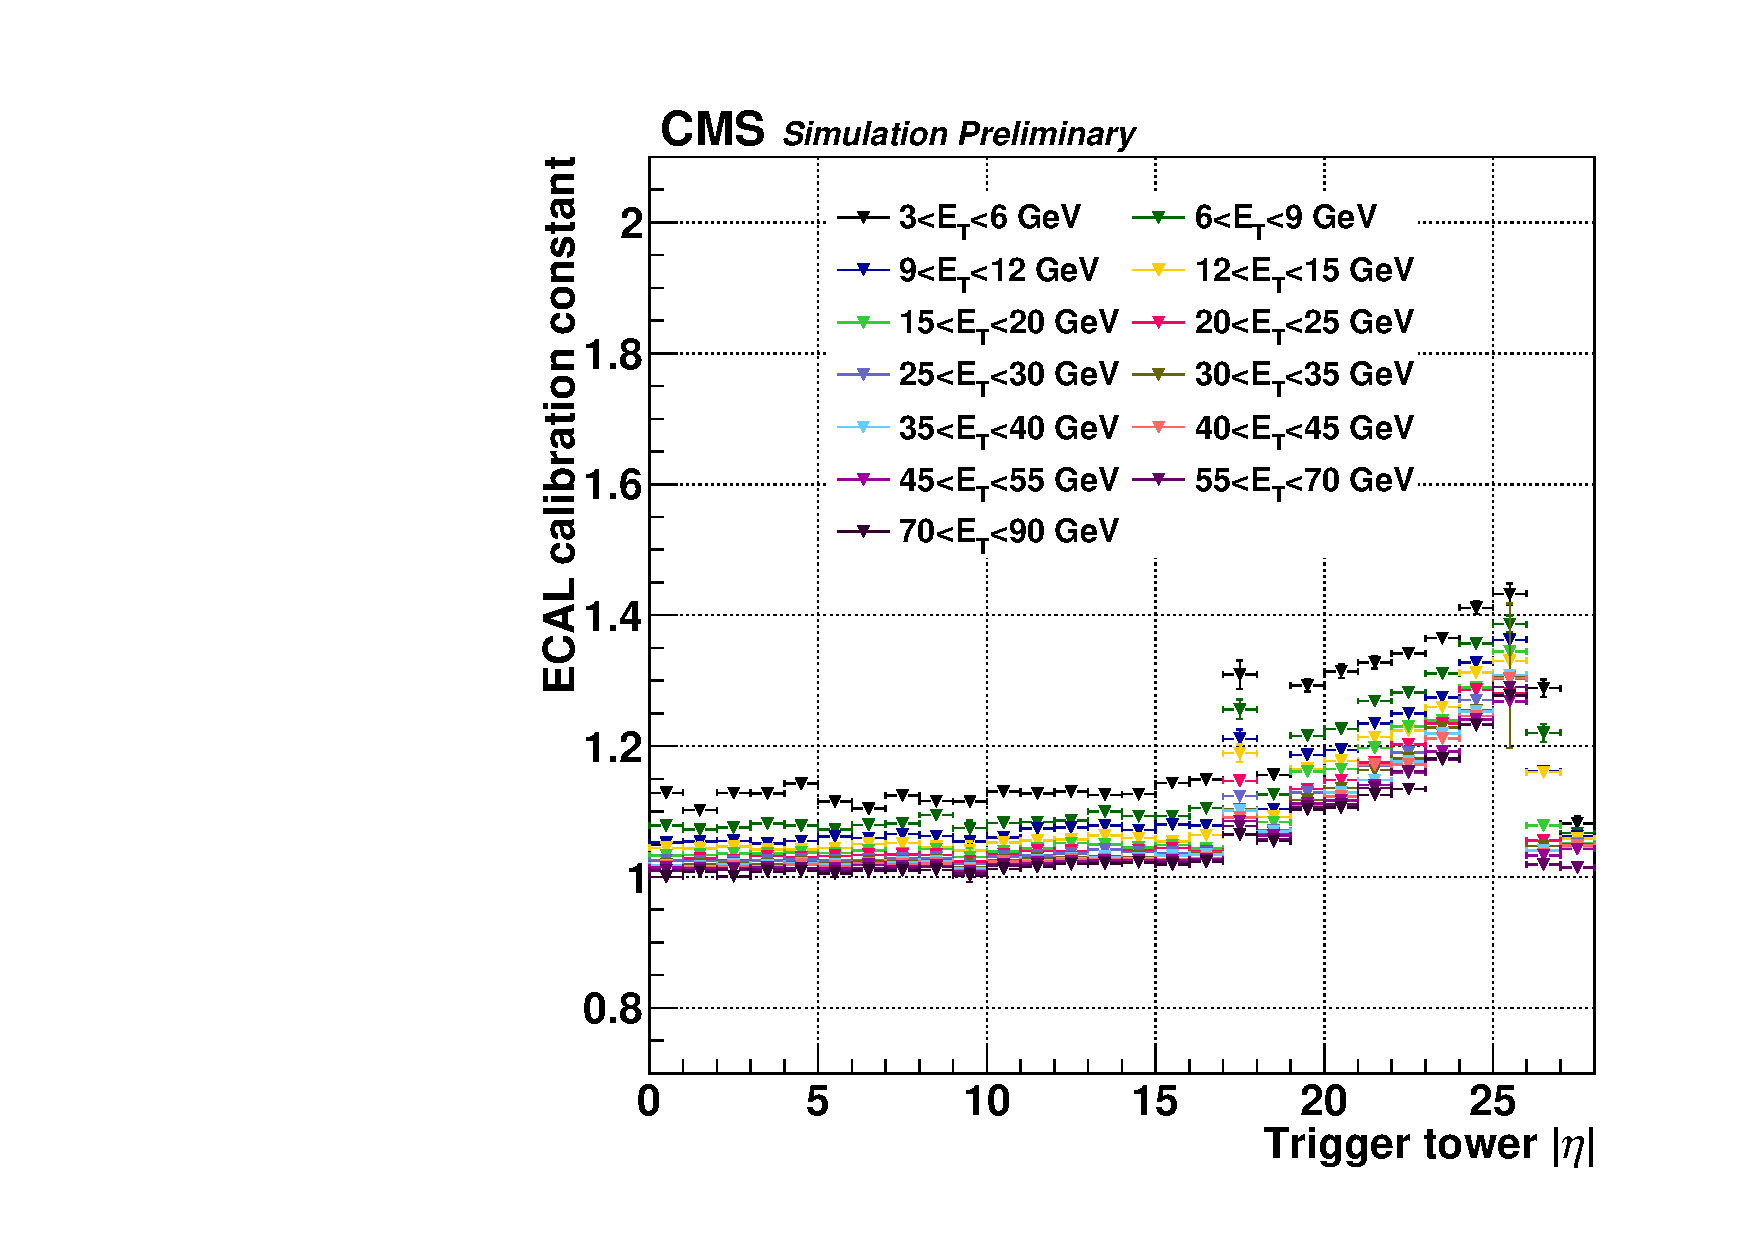
\includegraphics[width=0.49\textwidth]{Figures/photon_SF_3x3.pdf}
    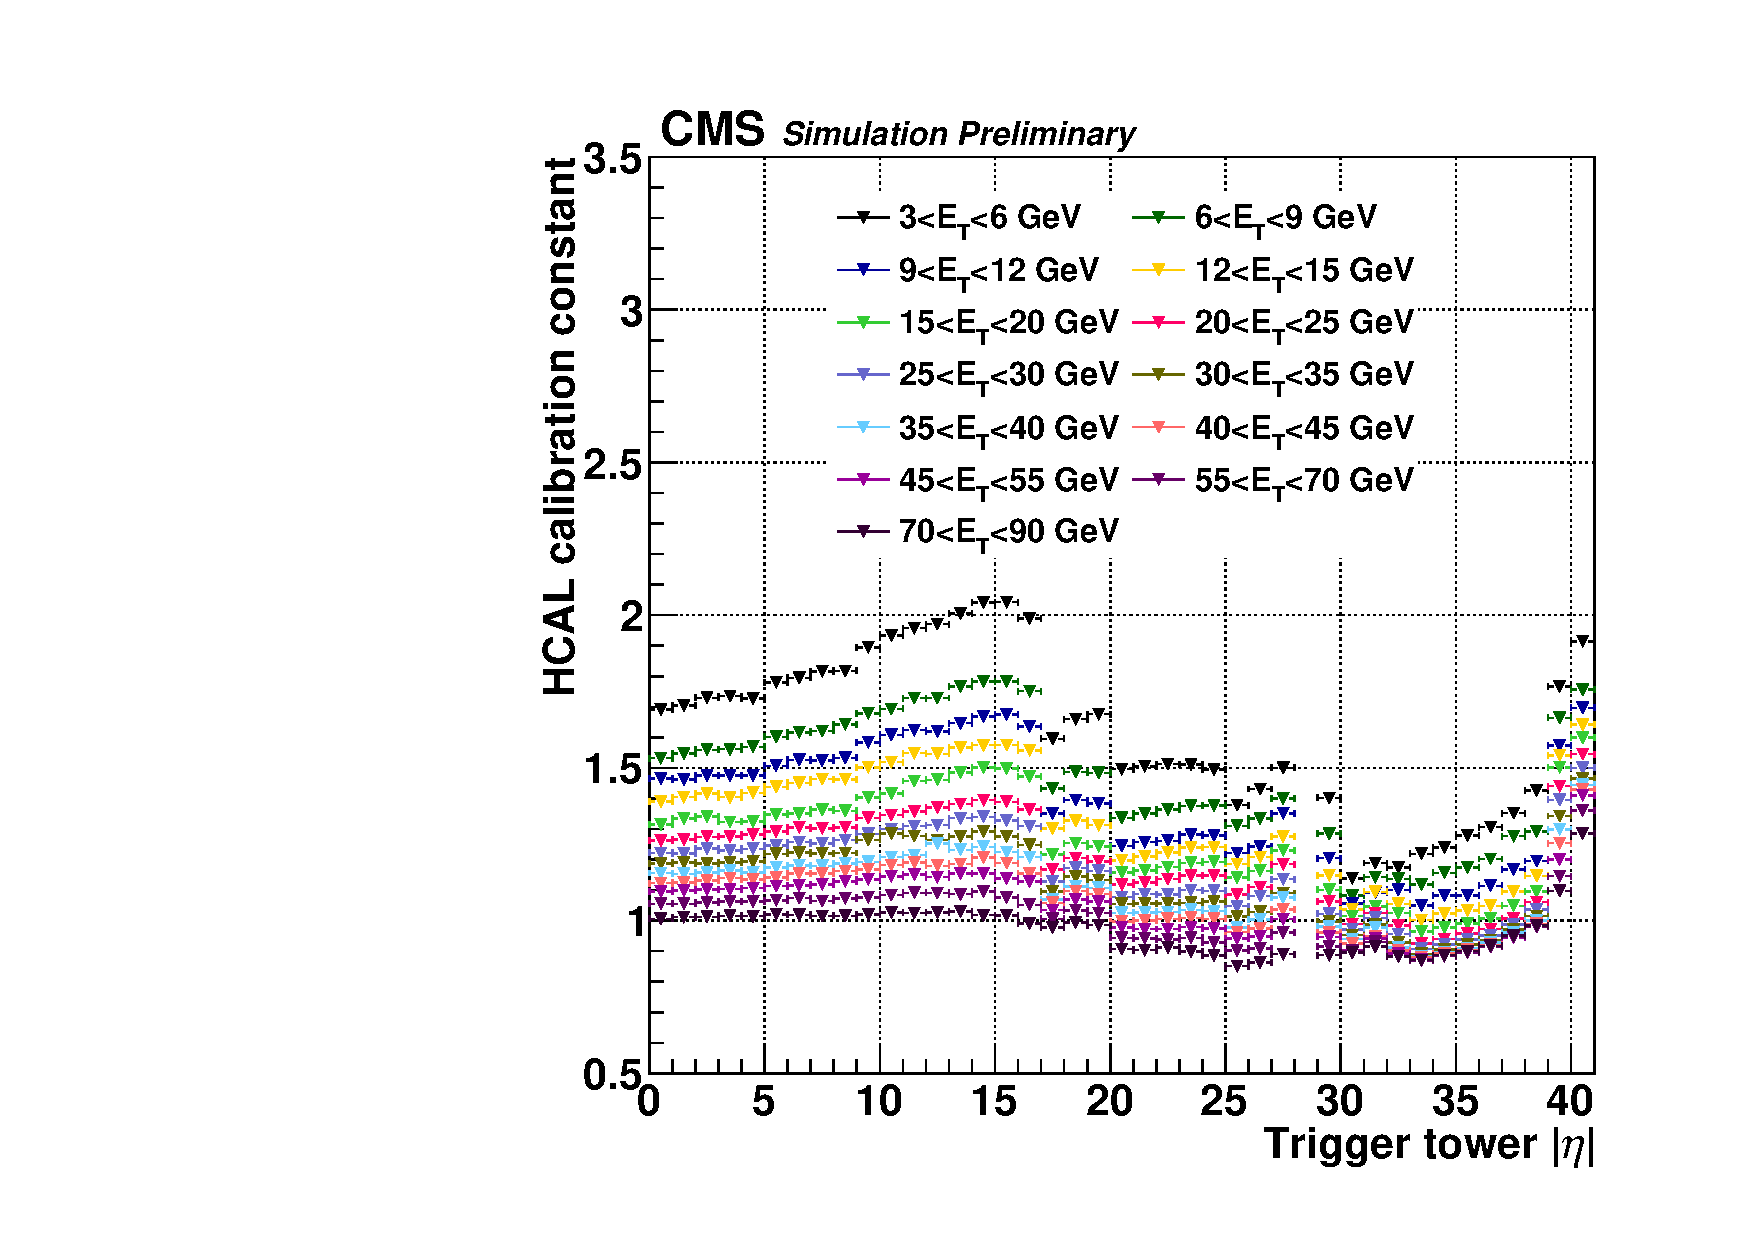
\includegraphics[width=0.49\textwidth]{Figures/picharged_SF_5x5.pdf}
    \caption{Calibration factors derived for Layer 1 of the calorimeter trigger, used in 2018 data taking. The energy of a trigger tower is multiplied
    by the scale factor corresponding to the tower's uncalibrated $E_{T}$ (color) and to the minimum number of other towers between it and $|\eta| = 0$ (x-axis).
    Calibrations were derived separately for the ECAL (left) and HCAL (right), using simulated photons and charged pions, respectively.}
    \label{fig:layer1_calibs}
  \end{center}
\end{figure}

The TPs from CSCs and DTs are track segments. Along with hits recorded in the RPCs, muon system TPs are routed through a lattice of preprocessor
layers and then sent to dedicated Barrel, Endcap, and Overlap Track Finders covering different $\eta$ regions.
These rapidly assemble L1 Muon objects and send them to the Global Muon Trigger,
which sorts the L1 Muons by $p_\mathrm{T}$ and quality, finally sending this information along to the GT.

The GT tests the L1 objects it receives against a set of L1 trigger paths, which specify various event selection criteria. After evaluating
which trigger paths have been passed, the GT makes the final L1A decision. The time from TP generation to L1A decision cannot be longer than
4\unit{\micro s}, and the overall L1A rate cannot be higher than 100\unit{kHz}; in 2016, this was the typical L1A rate actually achieved.

If the L1A is given, the full detector data is sent to the HLT, which consists of software running on commercial computing hardware.
The HLT tests each event against a set of high-level trigger paths. Each of these paths has access to raw detector information as well
as quantities computed at L1. Enough time and memory are available to perform a reduced sequence of the full offline event reconstruction
algorithms, separately optimized for each path. In 2016, the average HLT processing time per event was less than 160\unit{ms},
and the typical HLT accept rate was 1\unit{kHz}.

\subsection{Luminosity measurement} \label{sec:LHCCMS_CMS_lumi}
In principle, the integrated luminosity is given by integrating the instantaneous luminosity defined by Eq.~\ref{eq:instantaneous_lumi} over the data taking period,
with an extra efficiency factor to account for the fraction of time during which the trigger was active. In practice, the uncertainty on the
parameters of Eq.~\ref{eq:instantaneous_lumi} is fairly high, and more precise measurements of instantaneous luminosity are obtained by directly examining the beam intensities.

In the method developed
by van der Meer~\cite{ref:CERN-ISR-PO-68-31}, the two beams are scanned across each other in the transverse plane, giving a direct experimental
probe of the beam profile that is used to calibrate the relationship between instantaneous luminosity and specific observables accessible to various
beam monitoring instruments. A van der Meer scan establishes the calibrated visible cross section $\sigma_\mathrm{vis}$ of a process examined
by each luminometer, such that the instantaneous luminosity measured by a luminometer is given by
\begin{equation}
\mathcal{L} = R / \sigma_\mathrm{vis}
\label{eq:lumi_calibration}
\end{equation}
where $R$ is the observed rate of the process measured by the luminometer. The pixel tracker, DTs, and HF are used for this purpose, in addition to two
dedicated instruments: the Fast Beam Conditions Monitor (BCM1f) and Pixel Luminosity Telescope (PLT).

Van der Meer scans require dedicated LHC runs outside of normal data taking, but the calibrated luminometers continue to monitor the beam luminosity
during physics runs. The uncertainty on calibrated luminosity measurements in 2016 data taking is 2.5\%~\cite{ref:CMS-PAS-LUM-17-001}.
The data set used in this thesis corresponds to a time-integrated luminosity $L = 35.9\fbinv$.
